\setcounter{page}{1}
\section*{Zielsetzung}
Mit dem Versuch soll der Hall-Effekt durch Messung der 
Hall-Spannung experimentell bestätigt werden.

\section{Theorie}

\subsection{Elektrische Leitfähigkeit}
Jedes Atom besitzt nach der Quantenmechanik und dem Pauli-Prinzip 
Energiebänder.
Diese geben die für ein gebundenes Elektron möglichen Energiebereiche an. Auf den Bändern kann das Elektron weder 
Energie aufnehmen noch abgeben. Es kann also 
nicht beschleunigen bzw. abbremsen (z. B. durch ein äußeres E-Feld).
Lediglich bei leitenden Elementen (z. B. Metallen) gibt es ein sogenanntes \emph{Leitfähigkeitsband}.
Auf diesem besitzen die Elektronen (\emph{Leitungselektronen}) die Möglichkeit zu beschleunigen oder abzubremsen.
Bei Isolatoren befinden sich keine freien Elektronen auf dem \emph{Leitfähigkeitsband}.
In Metallen kommt es zu Bildung von Gitterstrukturen. 
Auf diesen verhalten sich die \emph{Leitungselektronen}, wie Teilchen eines idealen Gases.
Es es kommt unter den Elektronen zu Stoßvorgängen.
Die gemittelte Zeit zwischen zwei Stößen wird als \emph{mittlere Flugzeit} $\overline{\tau}$ bezeichnet.

Wird ein Elektron mittels $\vec{F}=\map{e}\vec{E}$ ($\map{e}\, \hat{=}$ Elementarladung) beschleunigt 
ergibt sich für \emph{Driftgeschwindigkeit}:

\begin{equation}
\label{eq:drift_v}
\vec{\overline{v}}\ua{d}=\frac{1}{2}\Delta\vec{v}=-\frac{1}{2}\frac{\map{e}}{\map{m}\ua{e}}\vec{E}\,\overline{\tau}
\end{equation}

Hierbei sei $\map{m}\ua{e}$ die Elektronenmasse.
Mittels der \emph{Driftgeschwindigkeit} kann nun auf die Stromdichte $j$ geschlossen werden. Dazu:

\begin{align}
j&=-n\overline{v}\ua{d}\map{e}=\frac{1}{2}\frac{\map{e^2}}{\map{m}\ua{e}}n E\overline{\tau}\notag \\
\Leftrightarrow \quad \overline{v}\ua{d}&=\frac{j}{n\map{e}}\label{eq:stromdicht}
\end{align}
Die Größe $n$ gibt die Anzahl der Elektronen pro Volumeneinheit an.
Mit der idealisierten Annahme eines homogenen Leiters wird, können 
$j=\frac{I}{Q}$ und $E=\frac{U}{L}$ umgeschrieben werden.
Dabei sei $Q$ der Querschnitt und $L$ die Länge des Leiters.
Mittels dem ohmschen Gesetz folgt anschließend

\begin{equation}
\label{eq:wider}
R=2\frac{\map{m}\ua{e}}{\map{e}^2}\frac{1}{n\overline{\tau}}\frac{L}{Q}
\end{equation}
\subsection{Der Hall-Effekt}
Der \emph{Hall-Effekt} kommt immer dann zu stande, wenn 
ein Magnetfeld senkrecht auf einer stromdruchflossene
homogen Leiterplatte (Dicke $d$ und Breite $b$) steht.
Die Lorentzkraft $\vec{F}\ua{l}$ sorgt für eine Ablenkung der Elektronen.
Die Ablenkung bewirkt eine Potentialdifferenz zwischen den 
Punkten $A$ und $B$ (vgl. \ref{}). Dadruch entsteht gleichzeitig ein
weiteres elektrisches Feld $E\ua{y}$, es wirkt der Elektronenbewegung entgegen.
Die Spannung zwischen $A$ und $B$ wächst so lange an, bis es zu einem Kräftegleichgewicht zwischen der Lorentz- und Coulombkraft kommt.
Die gemessene Hallspannung ist  dann gleich

\begin{equation}
\label{eq:hall_span}
U\ua{H}=E\ua{y}b=\overline{v}\ua{d}Bd=-\frac{1}{n\map{e}}\frac{BI\ua{q}}{d}
\end{equation}
Die Hallspannung kann also Auskunft über die Ladungsträgerdichte $n$ geben.
Den Gleichung \eqref{eq:hall_span} ist bei konstanter Stromstärke eine Geradengleichung der Form $U\ua{H}=mB$ mit
\begin{align}
m&=\frac{1}{n\map{e}}\frac{I\ua{q}}{d} \notag \\
\Leftrightarrow \quad n&=\frac{I\ua{q}}{m\map{e}d}\label{eq:steig_teil_anz}
\end{align}


\subsection{Berechnung mikroskopischer Leitfähigkeitsparameter}
Mithilfe des Widerstandes und der \emph{Hall-Spannung} kann nun auf 
einige mikroskopische Leitfähigkeitsparamete geschlossen werden.
Zum einen lässt sich die mittlere \emph{freie Weglänge} $\overline{l}$ bestimmen.
Dazu wird der Zusammenhang

\begin{equation*}
\label{eq:freie_weg}
\overline{l}=\overline{\tau}\left|\,v\,\right|
\end{equation*}
verwendet.
Es ist $\left|\,v\,\right|$ die Totalgeschwindigkeit des Elektrons.
Sie entsteht durch die Wärmebewegung der Kristallbausteine.
Um die Totalgeschwindigkeit eines Elektrons zu bestimmen, nutzt 
man die \emph{Fermie-Energie} $E\ua{F}$. Sie nimmt den Wert des energiereichsten Elektrons wegen des 
Pauli-Verbotes am absoluten Nullpunkt an.
Und wir mit dem Zusammenhang 

\begin{equation}
\label{eq:fermi_e}
E\ua{f}=\frac{h^2}{2\map{m}\ua{e}}\left[\left(\frac{3}{8\pi}\right)^2\right]^{\frac{1}{3}}
\end{equation}
berechnet. In Formel \eqref{eq:fermi_e} wird das Plancksches Wirkungsquantum $h$ benutzt.
Da kaum ein Elektron $E\ua{f}$ erreicht und somit im Wesentlichen nicht 
für die elektrische Leitfähigkeit verantwortlich ist.
Kann die Totalgeschwindigkeit abgeschätzt werden, mit

\begin{equation}
\label{eq:total_v}
\left|\,\overline{v}\,\right|\approx\left(\frac{2E\ua{F}}{\map{m}\ua{e}}\right)^{\frac{1}{2}}.
\end{equation}
Damit erhalten wir für die  mittlere \emph{freie Weglänge}:
\begin{equation}
\label{eq:mit_frei_weg}
\overline{l}\approx\overline{\tau}\sqrt{\frac{2E\ua{f}}{m\ua{e}}}
\end{equation}

Mittels der Flugzeit $\ov{\tau}$ wird die \emph{Beweglichkeit} $\mu$ errechnet,
dazu die Formel 

\begin{align}
\vec{\ov{v}}\ua{d}&=\mu\vec{E} \notag \\ 
\Leftrightarrow \quad \mu&=\frac{1}{2}\frac{\map{e}}{m\ua{e}} \label{eq:beweg}
\end{align}

\subsection{Hysterese} 

Die \emph{Hysterese} beschreibt die nicht lineare 
Abhängigkeit der magnetischen Flussdichte $B$ zu der 
magnetischen Feldstärke $H$. In Abbildung \ref{fig: hyste} ist 
diese Abhängigkeit in der Hysteresekurve zu sehen. 
Bei dem Versuch ist die sogenannte Remanenz zu beachten (in \ref{fig: hyste} $\map{P}_2$).
Sie steht für den Verbleib einer Remanent-Flussdichte bei $H=0$ (Restmagnetisierung).
Nur durch eine ausreichend großes Gegenfeld kann diese beseitigt werden.
Die von der Hysteresekurve eingeschlossene Fläche gibt die für die Magnetisierung benötigte
Arbeit an. Das Aufbringen der Energie sorgt, aber gleichzeitig für eine Erwärmung des Kernes.

\begin{figure}
  \centering
  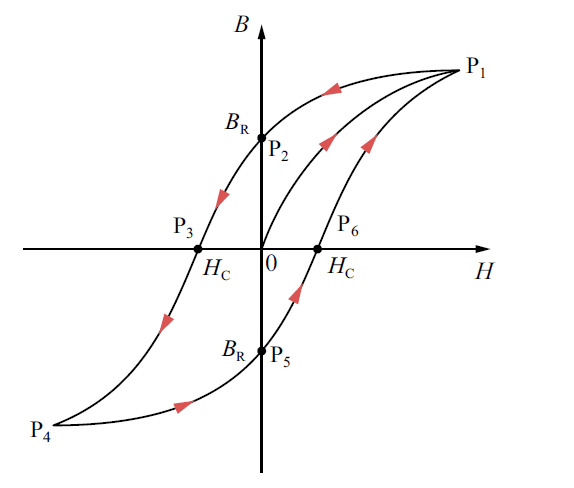
\includegraphics[width=0.5\textwidth]{pics/hystereskurve.png}
  \caption{Hysteresekurve \cite{hyste}}
  \label{fig: hyste}
\end{figure}
